\chapter{Data}

\section{Processing and Storage}

To facilitate the storage and processing of this large amount of data we used an AMD supercomputer with 64 cores. Inspired by the  map reduce paradigm we split the dataset into 64 parts and assigned each to a single core. To efficiently use the hardware resources we manually controlled for the memory assignment using numactl. As illustrated in\textbf{ \ref{fig:dataProcessing}} eight cores directly access one out of eight memory blocks. Each dataset was filtered in parallel reducing the 64 dataset to two lexicons. 

 \begin{figure}[H]
\centerline{ \noindent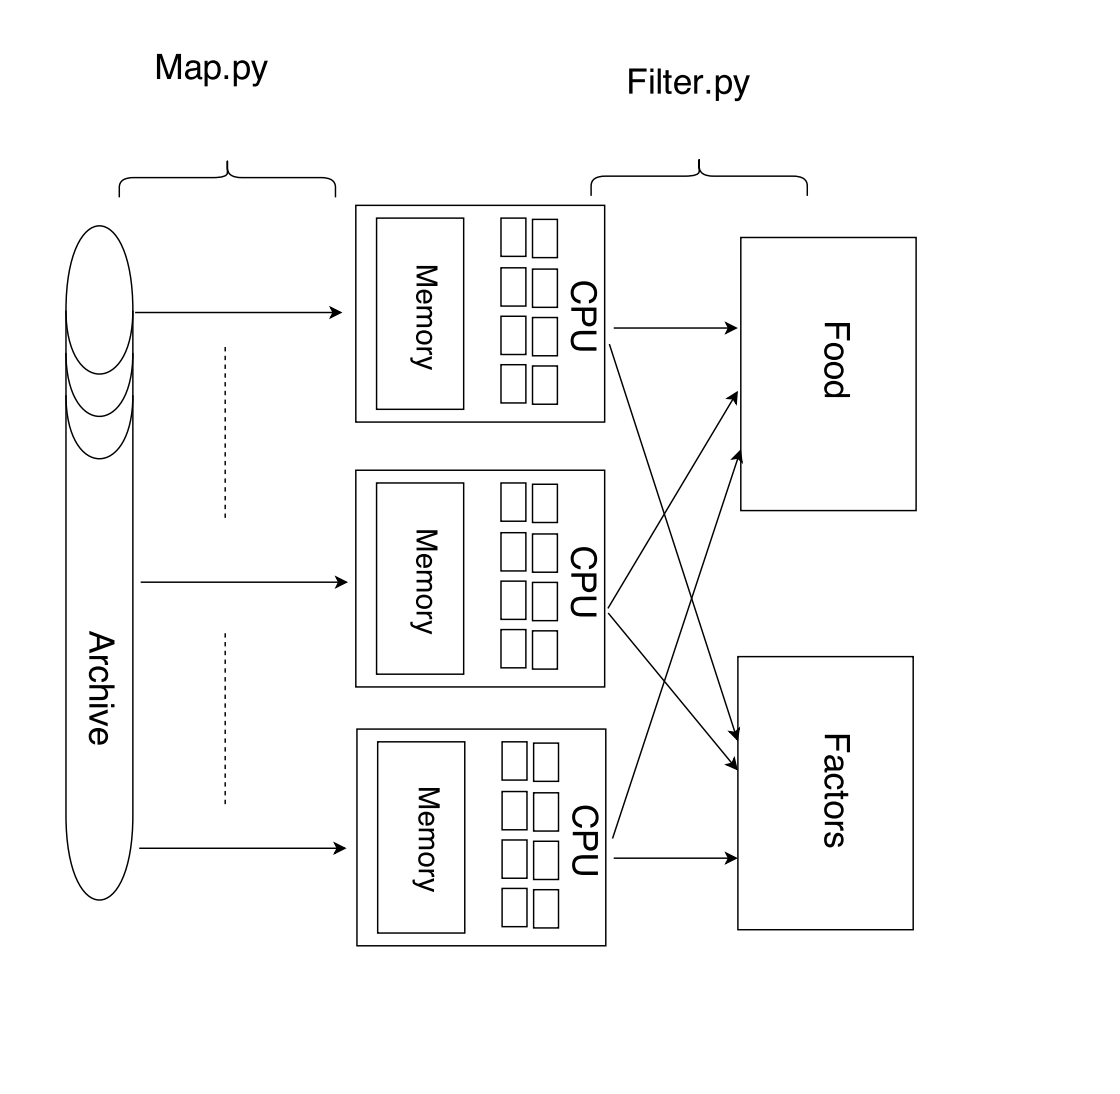
\includegraphics[width=0.8\textwidth]{img/abs/hw_model}}
 \caption{Dada Processing}
 \label{fig:dataProcessing}
\end{figure}

\section{Crowd Flower}

For the categorisation of the keywords for our predictor lexicon four crowd tasks were created. This section details the instructions given to the crowd workers for the four categorisation tasks. 

\subsection{Categorise: Food Price}

This is a categorization task centered around food security. Please categorize terms appearing in tweets about food in order to help us quantify users perception of Food Price. Overlaps may occur, i.e a term can potentially be indicative of both food price and food supply. Such keywords should always be classified as B. Likely .

Is the word or pair of words likely to be indicative of a user perception of food price?

A. YES, the term is indicative of food cost and/or can be used as a synonym of price

\begin{itemize}

  \item pricy 
  \item expensive 
  \item cheap 
  \item affordable 
  \item bill 
  \item receipt 
  \item cost 
\end{itemize}


B. LIKELY, the term might be indicative of food supply or food cost
\begin{itemize}
  \item low
  \item high 
  \item increasing 
\end{itemize}


C. NO, the term is unlikely to be indicative of food cost 
\begin{itemize}
  \item when
  \item chair
  \item boy
\end{itemize}


D. Not in English, not understandable, other issues.


\subsection{Categorise: Food Supply}

This is a categorization task centered around food security. Please categorize terms appearing in tweets about food in order to help us quantify users perception of Food Supply. Overlaps may occur, i.e a term can potentially be indicative of both food supply and food cost. Such keywords should always be classified as B. Likely.

Is the word or pair of words likely to be indicative of a user perception of food supply?


A. YES, the term is indicative of food supply


\begin{itemize}
  \item available 
  \item accessible 
    \item lack 
  \item amount 
  \item number 
   \item stock 
   \item ressource 
\end{itemize}

B. LIKELY, the term might be indicative of food supply or food cost
\begin{itemize}
  \item low
  \item high 
  \item increasing  
\end{itemize}

C. NO, the term is unlikely to be indicative of food supply 
\begin{itemize}
  \item when
  \item chair
  \item boy
\end{itemize}

D. Not in English, not understandable, other issues.



\subsection{Categorise: Food Poverty}

This is a categorisation task centered around food security. Please categorise terms appearing in tweets about food in order to help us quantify users perception of Food Poverty. Overlaps may occur, i.e a term can potentially be indicative of both food poverty and food needs. Such keywords should always be classified as B. Likely.

Is the word or pair of words likely to be indicative of a user perception of food poverty or the user perception of wealth?

A. YES, the term is indicative of food poverty or wealth

\begin{itemize}

  \item starving
  \item donation
  \item wealth 
  \item luxury
  \item profit
  \item help
  \item diabetes
  \item obesity
  \item healthy

\end{itemize}

B. LIKELY, the term might be indicative of food poverty and wealth or might be an indicator for food needs\begin{itemize}
  \item crave
  \item urgent
  \item must
  \item need 
\end{itemize}

C. NO, the term is unlikely to be indicative of food poverty or wealth

\begin{itemize}
  \item when
  \item chair
  \item boy
\end{itemize}

D. Not in English, not understandable, other issues.



\subsection{Categorise: Food Needs}

This is a categorization task centered around food security. Please categorize terms appearing in tweets about food in order to help us quantify users perception of Food Needs. Overlaps may occur, i.e a term can potentially be indicative of both food needs and food poverty. Such keywords should always be classified as B. Likely .

Is the word or pair of words likely to be indicative of a user perception of food needs?

A. YES, the term is indicative of food needs

\begin{itemize}
  \item love
  \item want
  \item hate
  \item favorite 
  \item satisfied
  \item foodporn
  \item yum


\end{itemize}

B. LIKELY, the term might be indicative of food needs or food poverty
\begin{itemize}
  \item crave
  \item urgent
  \item must
  \item need
\end{itemize}

C. NO, the term is unlikely to be indicative of food needs 
\begin{itemize}
  \item when
  \item chair
  \item boy
\end{itemize}

D. Not in English, not understandable, other issues.

